\section{Topic models and their evaluations}
\label{sec:models}
%% \subsection{Topic models in a nutshell}

% Topic models discover patterns of word usage in a corpus.  Related
% words often appear in similar documents, and topic models can discover
% clusters of words that share context.  Because words in these clusters
% often seem to ``make sense'' together, they are described as topics.
% For illustration, three topics from a topic model called latent
% Dirichlet allocation (LDA)~\cite{blei-03} are shown in
% Figure~\ref{fig:nyttopics:topic}.

% Topic models are unsupervised; they do not require labels or
% annotations.  Instead, they discover latent topics directly from the
% data.  In addition to finding topics, topic models also assign
% mixtures of these topics to documents.  This is illustrated in
% Figure~\ref{fig:nyttopics:doc}. 

% We restrict ourselves to exchangeable topic models, in which the order
% of the words within a document does not matter.  The models we
% consider are also probabilistic, in the sense that they seek to
% approximate the vector of observed word counts as a mixture of topic
% distributions; fitting one of these topic models entails finding a
% point on the topic simplex that best describes the document.

Topic models posit that each document is expressed as a mixture of
topics.  These topic proportions are drawn once per document, and the
topics are shared across the corpus.  In this paper we will consider
topic models that make different assumptions about the topic
proportions.  Probabilistic Latent Semantic Indexing
(pLSI)~\cite{hofmann-99} makes no assumptions about the document topic
distribution, treating it as a distinct parameter for each document.
Latent Dirichlet allocation (LDA)~\cite{blei-03} and the correlated
topic model (CTM)~\cite{blei-06} treat each document's topic
assignment as a multinomial random variable drawn from a symmetric
Dirichlet and logistic normal prior, respectively.

While the models make different assumptions, inference algorithms for all of
these topic models build the same type of latent space: a collection of topics
for the corpus and a collection of topic proportions for each of its
documents.  While this common latent space has explored for over two decades,
its interpretability remains unmeasured.

\begin{figure*}[t]
\centering
%  \hspace{-5cm}
\subfigure[Topics]{
  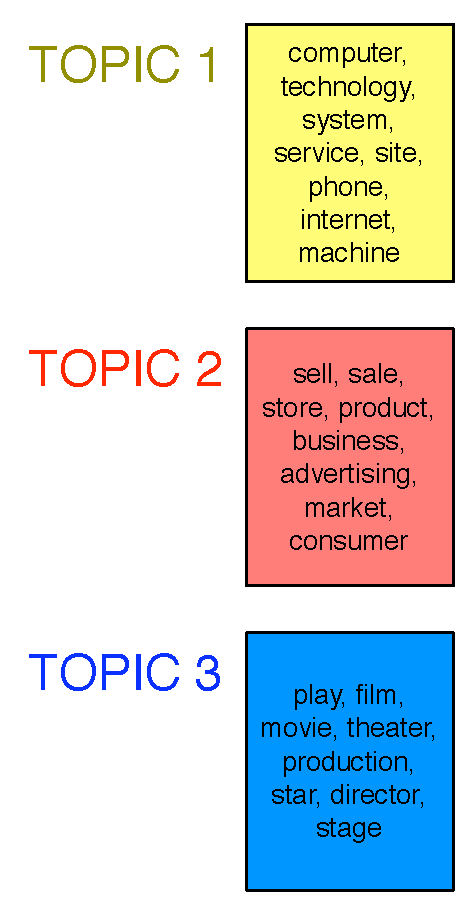
\includegraphics[scale=0.35]{figures/nyt_topics.pdf}
  \label{fig:nyttopics:topic}
}
\hspace{0.4in}
\subfigure[Document Assignments to Topics]{
  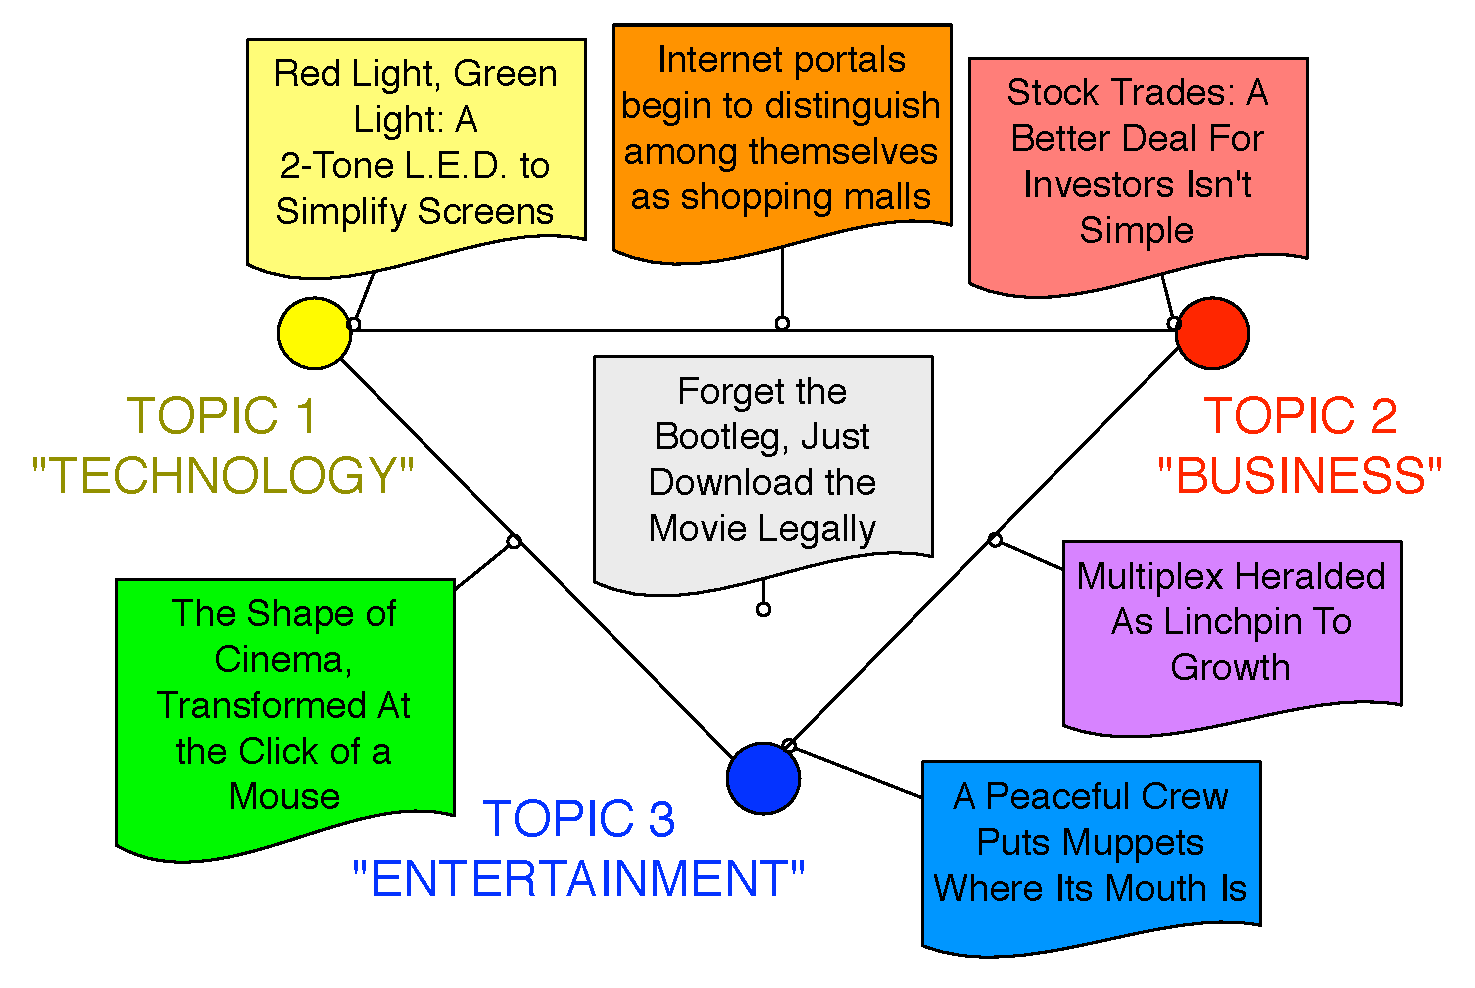
\includegraphics[scale=0.35]{figures/nyt_documents.pdf}
  \label{fig:nyttopics:doc}
}
\caption{The latent space of a topic model consists of topics,
  which are distributions over words, and a distribution over these
  topics for each document.  On the left are three topics from a
  fifty topic LDA model trained on articles from the New York
  Times.  On the right is a simplex depicting the distribution
  over topics associated with seven documents.  The line from each
  document's title shows the document's position in the topic
  space.}
\label{fig:nyttopics:big}
\end{figure*}


% cw: i mask the following paragraph, it seems duplicated with the next subsection

%Because the field of topic models is so vibrant, we cannot mention
%every variant or application.  Considered broadly, topic models
%encompass everything from a mixture of unigrams~\cite{Nigam-00} to
%hierarchical non-parametric methods~\cite{blei-07} and have found
%applications in collaborative filtering~\cite{Marlin:2004}, computer
%vision~\cite{feifei:hdp}, and genetics~\cite{populationstructure}.

% jbg: More detail about LDA / CTM?  I'll leave that until later, I guess.

% jbg: I had originally planned to put in DTM, SLDA, etc. here, but
% now I'm thinking that would distract from the flow.  Perhaps that
% best belongs in the intro?


% An introduction to topic models must begin with latent semantic
% analysis , which came from the psychology
% community.  Although we focus on later probabilistic topic models, LSA
% laid the foundation for those models and set important precedents for
% evaluation, so we briefly mention its assumptions.  LSA represents a
% corpus as a matrix $X$ where $X_{i,j}$ is the number of times word $j$
% appears in document $j$.  This matrix is then approximated using
% singular value decomposition.

\subsection*{Pay no attention to the latent space behind the model}

Although we focus on probabilistic topic models, the field began in
earnest with latent semantic analysis (LSA)~\cite{landauer-97}.  LSA,
the basis of pLSI's probabilistic formulation, uses linear algebra to
decompose a corpus into its constituent themes.  Because LSA
originated in the psychology community, early evaluations focused on
replicating human performance or judgments using LSA: matching
performance on standardized tests, comparing sense distinctions, and
matching intuitions about synonymy (these results are reviewed
in~\cite{landauer-02}).  In information retrieval, where LSA is known
as latent semantic indexing (LSI)~\cite{deerwester-90}, it is able to
match queries to documents, match experts to areas of expertise, and
even generalize across languages given a parallel
corpus~\cite{berry-95}.

The reticence to look under the hood of these models has persisted
even as models have moved from psychology into computer science with
the development of pLSI and LDA.  Models either use measures based on
held-out likelihood~\cite{blei-03,blei-06} or an external task that is
independent of the topic space such as sentiment
detection~\cite{titov-08} or information retrieval~\cite{wei-06}.
This is true even for models engineered to have semantically coherent
topics~\cite{boyd-graber-07}.

For models that use held-out likelihood, Wallach et
al.~\cite{wallach-09} provide a summary of evaluation
techniques. These metrics borrow tools from the language modeling
community to measure how well the information learned from a corpus
applies to unseen documents.  These metrics generalize easily and
allow for likelihood-based comparisons of different models or
selection of model parameters such as the number of topics.  However,
this adaptability comes at a cost: these methods only measure the
probability of observations; the internal representation of the models
is ignored.

Griffiths et al.~\cite{griffiths-06} is an important exception to the
trend of using external tasks or held-out likelihood.  They showed
that the number of topics a word appears in correlates with how many
distinct senses it has and reproduced many of the metrics used in the
psychological community based on human performance.  However, this is
still not a deep analysis of the structure of the latent space, as it
does not examine the structure of the topics themselves.

We emphasize that not measuring the internal representation of topic
models is at odds with their presentation and development.  Most topic
modeling papers display qualitative assessments of the inferred topics
or simply assert that topics are semantically meaningful, and
practitioners use topics for model checking during the development
process.  Hall et al.~\cite{hall-08}, for example, used latent topics
deemed historically relevant to explore themes in the scientific
literature.  Even in production environments, topics are presented as
themes: Rexa (http://rexa.info), a scholarly publication search
engine, displays the topics associated with documents.  This implicit
notion that topics have semantic meaning for users has even
motivated work that attempts to automatically label
topics~\cite{mei-07}.  Our goal is to measure the success of
interpreting topic models across number of topics and modeling
assumptions.


% jbg: Does JSTOR have something we can cite yet?

% dmb: above, i think that rexa etc should be cited earlier. (see the
% dmb in the intro.)  i wonder if a variant of that last paragraph can
% appear in the introduction and then merely be reiterated here.  this
% is on p3, which isn't so bad, but p1 is better.

%\subsection{Examining Topic Coherence and Document Relevance}
%\label{sec:coherence}
